\subsubsection{Task realization}
For this task I used Qt Creator IDE. At the beggining I designed window using graphical drag \& drop staff from \textbf{Design} tab.
I added buttons for digits, required operations, and additionally an 'C' button, to erase current operand and also for getting
full grid 4 by 5 buttons. Of course an Text Edit box(with disabled editing). Figure \ref{fig:design} shows screenshot of finished
window. Red boxes are grid auto alignments.
\begin{figure}[H]
    \centering
    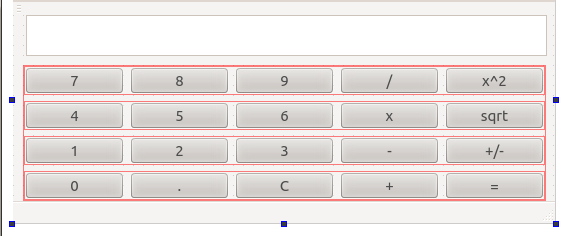
\includegraphics[width=0.9\textwidth]{screen1.png}
    \caption{Design}
    \label{fig:design}
\end{figure}

After that, I started adding slots, and adding connections from \texttt{clicked()} signal to window. All digits I connected 
to the same slot, \texttt{digitClicked}
\begin{verbatim}
   void MainWindow::digitClicked(){
    QPushButton *clickedButton = qobject_cast<QPushButton *>(sender());
    int digitValue = clickedButton->text().toInt();
    if(ui->summator->toPlainText() == "0" && digitValue==0.0)
        return;
    if (waitingForOperand) {
        ui->summator->clear();
        waitingForOperand = false;
    }
    ui->summator->setText(ui->summator->toPlainText() + QString::number(digitValue));
} 
\end{verbatim}
We get necessary digit from \texttt{text().toInt();} of the sender, because we know that sender will be a button, and it's 
text field is equal to value of the digit. \texttt{ui->summator} actually is display of our calculator, I'm too lazy to find
a prettier way to access it. Of course it can be declared as a field of MainWindow class, but ui is already a member, so it 
will become redundant. 

\begin{figure}[H]
    \centering
    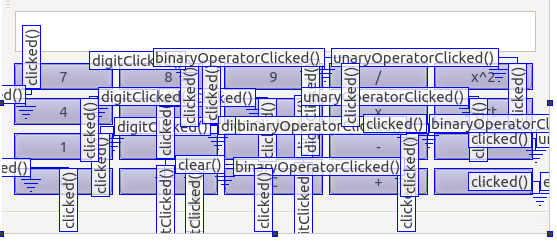
\includegraphics[width=0.9\textwidth]{screen2.png}
    \caption{Connected signals}
    \label{fig:signals}
\end{figure}

After connecting the signals(see Figure \ref{fig:signals}, it is messy because there are lot of signals and not so much space) 
 and testing input, I proceeded with simplest operations, unary, because you need just one operand.
\begin{verbatim}
void MainWindow::unaryOperatorClicked(){
    QPushButton *clickedButton = qobject_cast<QPushButton *>(sender());
    QString clickedOperator = clickedButton->text();
    double operand = ui->summator->toPlainText().toDouble();
    double result = 0.0;

    if (clickedOperator == tr("sqrt")) {
        result = sqrt(operand);
    }
    else if (clickedOperator == tr("x^2")){
        result = pow(operand, 2.0);
    }
    else if (clickedOperator == tr("+/-")){
        result = -operand;
    }
    ui->summator->setText(QString::number(result));
    waitingForOperand = true;
}
\end{verbatim}
There is no check, but in case of division by zero in UI will be displayed \emph{Inf}, in case of square root from negative - \emph{NaN}.
Also it would look clearer with switch-case construct, but from some strange reason Qt seems to accept \texttt{switch} only on integers.

In case of binary operation, we store curent value, store operation, and wait next operand. When clicking on equal - the 
operand and operation from the class atributes will be used:
\begin{verbatim}
void MainWindow::binaryOperatorClicked(){
    QPushButton *clickedButton = qobject_cast<QPushButton *>(sender());
    QString clickedOperator = clickedButton->text();
    double operand = ui->summator->toPlainText().toDouble();
    ui->summator->setText("0");
    sumInMemory=operand;
    pendingOperator=clickedOperator;
    waitingForOperand = true;
}

void MainWindow::equalClicked(){
    double operand = ui->summator->toPlainText().toDouble();
    double result = 0.0;
    if (pendingOperator=="/") result = sumInMemory/operand;
    else if (pendingOperator=="-") result = sumInMemory-operand;
    else if (pendingOperator=="+") result = sumInMemory+operand;
    else if (pendingOperator=="x") result = sumInMemory*operand;

    ui->summator->setText(QString::number(result));
    sumInMemory=0.0;
    waitingForOperand = true;
}
\end{verbatim}

For consistent conversion to double, point will be appendend to display value only in case if it isn't already present:
\begin{verbatim}
if (!ui->summator->toPlainText().contains("."))
    ui->summator->setText(ui->summator->toPlainText() + tr("."));
\end{verbatim}


\begin{figure}[H]
    \centering
    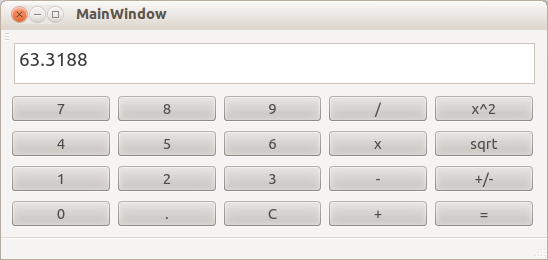
\includegraphics[width=0.9\textwidth]{screen3.png}
    \caption{Working application}
\end{figure}


